\section{The Adjoint of a Linear Operator} \label{sec 6.3}

\begin{remark} \label{remark 6.3.1}
It seems that this section is essentially related to the concept of \emph{dual space}, that is, \SEC{2.6}.
But we can still study this section directly.
\end{remark}

In \SEC{6.1}, we defined the conjugate transpose (see \DEF{6.2}) \(A^*\) of a matrix \(A\).
For a linear operator \(\T\) on an inner product space \(\V\), we now define a related linear operator on \(\V\) called the \emph{adjoint} of \(\T\), whose matrix representation with respect to \emph{any orthonormal} basis \(\beta\) for \(\V\) is \([\T]^*_{\beta}\).
The analogy between conjugation of complex numbers and adjoints of linear operators will become apparent. (See \THM{6.11}.)
We first need a preliminary result.
Let \(\V\) be an inner product space, and let \(y \in \V\).
The function \(g: \V \to F\) defined by \(g(x) = \LG x, y \RG\) is clearly linear, since inner product is linear on first component.
That is,
\begin{align*}
    g(cx + z, y) & = \LG cx + z, y \RG \\
        & = c \LG x, y \RG + \LG z, y \RG & \text{by \DEF{6.1}(a)(b)} \\
        & = c g(x) + g(z)
\end{align*}
More interesting is the fact that if \(\V\) is \emph{finite}-dimensional, \emph{every} linear transformation from \(\V\) into \(F\) \emph{is of this form}.

\begin{note}
看來無限維內積空間的線性泛函(linear function)又有反例?
\end{note}

\begin{theorem} \label{thm 6.8}
Let \(\V\) be a \emph{finite}-dimensional inner product space over \(F\), and let \(g: \V \to F\) be a \LTRAN{}.
Then there \emph{exists} a \textbf{unique} vector \(y \in \V\) such that \(g(x) = \LG x, y \RG\) for all \(x \in \V\).
\end{theorem}

\begin{proof}
Let \(\beta = \{ v_1, v_2, ..., v_n \}\) be an \emph{orthonormal} basis for \(\V\), and let
\[
    y = \sum_{i = 1}^n \conjugatet{g(v_i)} v_i.
\]
Define \(h: \V \to F\) by \(h(x) = \LG x, y \RG\), which is clearly linear.
Furthermore, for \(1 \le j \le n\) we have
\begin{align*}
    h(v_j) & = \LG v_j, y \RG = \LG v_j, \sum_{i = 1}^n \conjugatet{g(v_i)} v_i \RG & \text{by def of \(h\) and \(y\)} \\
        & = \sum_{i = 1}^n g(v_i) \LG v_j, v_i \RG & \text{since \(\InnerOp\) is \emph{conjugate} linear} \\
        & = g(v_{\RED{j}}) \LG v_j, v_{\RED{j}} \RG = g(v_j) \cdot 1 = g(v_j) & \text{since \(\beta\) is orthonormal}
\end{align*}
Since \(g\) and \(h\) agree on \(\beta\), we have that \(g = h\) (by \CORO{2.6.1}).

To show that \(y\) is unique, suppose that \(g(x) = \LG x, y' \RG\) for all \(x\).
Then \(\LG x, y \RG = \LG x, y' \RG\) for all \(x\);
so by \THM{6.1}(e), we have \(y = y'\).
\end{proof}

\begin{example} \label{example 6.3.1}
Define \(g : \SET{R}^2 \to \SET{R}\) by \(g(a_1, a_2) = 2a_1 + a_2\); clearly \(g\) is a \LTRAN{}.
Let \(\beta = \{ e_1, e_2 \}\), the standard ordered (orthonormal) basis.
So as the proof of \THM{6.8}, let \(y = \conjugatet{g(e_1)}e_1 + \conjugatet{g(e_2)}e_2 = \conjugatet{2} e_1 + \conjugatet{1} e_2 = (2, 1)\).
Then for any \((a_1, a_2) \in \SET{R}^2\) we have \(\LG (a_1, a_2), y \RG = \LG (a_1, a_2), (2, 1) \RG = 2 a_1 + a_2 = g(a_1, a_2)\), satisfying \THM{6.8}.
\end{example}

\begin{theorem} \label{thm 6.9}
Let \(\V\) be a \emph{finite}-dimensional inner product space, and let \(\T\) be a linear operator on \(\V\).
Then there \emph{exists} a \textbf{unique} function \(\T^*: \V \to \V\) such that \(\LG \T(x), y \RG = \LG x, \T^*(y) \RG\) for all \(x, y \in \V\).
Furthermore, \(\T^*\) is linear.
\end{theorem}

\begin{proof}
Let \(y \in \V\).
Define \(g: \V \to F\) by \(g(x) = \LG \T(x), y \RG\) for all \(x \in \V\).
We first show that \(g\) is linear.
Let \(x_1, x_2 \in \V\) and \(c \in F\).
Then
\begin{align*}
    g(c x_1 + x_2) & = \LG \T(c x_1 + x_2), y \RG & \text{by def of \(g\)} \\
        & = \LG c\T(x_1) + \T(x_2), y \RG & \text{since \(\T\) is linear} \\
        & = c \LG \T(x_1), y \RG + \LG \T(x_2), y \RG & \text{since \(\InnerOp\) is linear in first component} \\
        & = c g(x_1) + g(x_2). & \text{by def of \(g\)}
\end{align*}
Hence \(g\) is linear.

Since \(g\) is linear, we now apply \THM{6.8} to obtain a \textbf{unique} vector \(y' \in \V\) such that \(g(x) = \LG x, y' \RG\) for all \(x \in \V\);
that is, \(\LG \T(x), y \RG = \LG x, y' \RG\) \MAROON{(1)} for all \(x \in \V\).

Currently, given any \(y \in \V\), we derive a unique \(y' \in \V\), \textbf{so essentially this whole process can be used to define another function}, so
defining \(\T^*: \V \to \V\) by \(\T^*(y) = y'\).
Then from \MAROON{(1)} we have \(\LG \T(x), y \RG = \LG x, \T^*(y) \RG\) \MAROON{(2)}, and this is the equation we want \(\T^*\) to satisfy.

Finally, we will show that \(\T^*\) is linear and unique.
To show that \(\T^*\) is linear, let \(y_1, y_2 \in \V\) and \(c \in F\).
Then for any \(x \in \V\), we have
\begin{align*}
    & \LG x, \T^*(c y_1 + y_2) \RG = \LG \T(x), c y_1 + y_2 \RG & \text{by \MAROON{(2)}} \\
    & = \conjugatet{c} \LG \T(x), y_1 \RG + \LG \T(x), y_2 \RG & \text{since \(\InnerOp\) is conjugate linear in second component} \\
    & = \conjugatet{c} \LG x, \T^*(y_1) \RG + \LG x, \T^*(y_2) \RG & \text{by \MAROON{(2)} again} \\ 
    & = \LG x, c \T^*(y_1) + \T^*(y_2) \RG. & \text{by conjugate linear again}
\end{align*}
Since \(x\) is arbitrary, by \THM{6.1}(e), \(\T^*(c y_1 + y_2) = c\T^*(y_1) + \T^*(y_2)\), hence \(\T^*\) is linear.

Finally, we need to show that \(\T^*\) is unique. Suppose that \(\U: \V \to \V\) is linear and that it satisfies \(\LG \T(x), y \RG = \LG x, \U(y) \RG\) for all \(x, y \in \V\).
Then by \MAROON{(2)}, \(\LG x, \T^*(y) \RG = \LG x, \U(y) \RG\) for all \(x, y \in \V\), so again by \THM{6.1}(e), \(\T^* = \U\).
\end{proof}

\begin{additional definition} \label{adef 6.4}
The linear operator \(\T^*\) described in \THM{6.9} is called the \textbf{adjoint} of the operator \(\T\).
The symbol \(\T^*\) is read ``\(\T\) star.''
\end{additional definition}

\begin{remark} \label{remark 6.3.2}
Thus (given a linear operator \(\T\) on \(\V\),) \(\T^*\) is the \emph{unique} operator on \(\V\) satisfying \(\LG \T(x), y \RG = \LG x, \T^*(y) \RG\) for all \(x, y \in \V\).
Note that we also have
\begin{align*}
    \LG x, \T(y) \RG & = \conjugatet{\LG \T(y), x \RG} & \text{by \DEF{6.1}(c)} \\
    & = \conjugatet{\LG y, \T^*(x) \RG} & \text{by \THM{6.9}} \\
    & = \LG \T^*(x), y \RG; & \text{by \DEF{6.1}(c) again}
\end{align*}
so \(\LG x, \T(y) \RG = \LG \T^*(x), y \RG\) for all \(x, y \in \V\).
We may \textbf{view these equations symbolically} as \textbf{adding a \(*\) to \(\T\) when shifting its position} inside the inner product symbol.
\end{remark}

\begin{remark} \label{remark 6.3.3}
For an \emph{infinite}-dimensional inner product space, the adjoint of a linear operator \(\T\) may be defined to be the function \(\T^*\) such that \(\LG \T(x), y \RG = \LG x, \T^*(y) \RG\) for all \(x, y \in \V\), \textbf{provided it exists}.
Although the uniqueness and linearity of \(\T^*\) follow as before, \emph{the existence of the adjoint is not guaranteed} (see \EXEC{6.3.24}).
\textit{The reader should observe the necessity of the hypothesis of finite-dimensionality in the proof of \THM{6.8}}.
Many of the theorems we prove about adjoints, nevertheless, do not depend on \(\V\) being finite-dimensional.
\end{remark}

The next theorem is a useful result for \emph{computing} adjoints (operators).

\begin{theorem} \label{thm 6.10}
Let \(\V\) be a finite-dimensional inner product space, and let \(\beta\) be an \textbf{orthonormal} basis for \(\V\).
If \(\T\) is a linear operator on \(\V\), then
\[
    [\T^*]_{\beta} = [\T]^*_{\beta}.
\]
That is, the matrix representation of the adjoint of \(\T\) (on orthonormal basis \(\beta\)) is equal to the adjoint of matrix (see \DEF{6.2}) representation of \(\T\) (on \(\beta\)).
\end{theorem}

\begin{proof}
Let \(A = [\T]_{\beta}, B = [\T^*]_{\beta}\), and \(\beta = \{ v_1, v_2, ..., v_n \}\) be a orthonormal basis; we have to show \(B = A^*\).
Then for all \(i, j\),
\begin{align*}
    B_{ij} & = \LG \T^*(v_j), v_i \RG & \text{by \CORO{6.5.1}} \\
        & = \conjugatet{\LG v_i, \T^*(v_j) \RG} & \text{by \DEF{6.1}(c)} \\
        & = \conjugatet{\LG \T(v_i), v_j \RG} & \text{by \THM{6.9}} \\
        & = \conjugatet{A_{ji}} & \text{by \CORO{6.5.1} again} \\
        & = (A^*)_{ij} & \text{by \DEF{6.2}}
\end{align*}
Hence \(B = A^*\).
\end{proof}

\begin{corollary} \label{corollary 6.10.1}
Let \(A\) be an \(n \X n\) matrix.
Then \(\LMTRAN_{A^*} = (\LMTRAN_A)^*\).
That is, the left multiplication of \(A^*\) is equal to the adjoint of the left multiplication of \(A\).
\end{corollary}

\begin{proof}
Let \(\beta\) is the standard ordered basis for \(F^n\), in particular \(\beta\) is orthonormal.
Hence
\begin{align*}
    [(\LMTRAN_A)^*]_{\beta} & = ([\LMTRAN_A]_{\beta})^* & \text{by \THM{6.10}} \\
    & = A^* & \text{by \THM{2.15}(a)} \\
    & = [\LMTRAN_{A^*}]_{\beta} & \text{by \THM{2.15}(a) again} 
\end{align*}
So \((\LMTRAN_A)^*\) and \(\LMTRAN_{A^*}\) have the same matrix representation, hence they are equal to each other.
\end{proof}

As an illustration of \THM{6.10}, we compute the adjoint of a specific linear operator.
\begin{example} \label{example 6.3.2}
Let \(\T\) be the linear operator on \(\SET{C}^2\) defined by \(\T(a_1, a_2) = (2\iu a_1 + 3a_2, a_1 - a_2)\).
If \(\beta\) is the standard ordered basis for \(\SET{C}^2\),
then
\[
    [\T]_{\beta} = \begin{pmatrix}
        2 \iu & 3 \\ 1 & -1
    \end{pmatrix}.
\]
So by \THM{6.10}
\[
    [\T^*]_{\beta} = [\T]_{\beta}^* = \begin{pmatrix}
        -2 \iu & 1 \\ 3 & -1
    \end{pmatrix}.
\]
So converting the representation back, we have
\[
    \T^*(a_1, a_2) = (-2\iu a_1 + a_2, 3 a_1 - a_2).
\]
\end{example}

The following theorem suggests an \emph{analogy} between the \emph{conjugates} of complex numbers \emph{and the adjoints} of linear operators.

\begin{theorem} \label{thm 6.11}
Let \(\V\) be an inner product space, and let \(\T\) and \(\U\) be linear operators on \(\V\) whose adjoints \emph{exist}.
(So that we do not care the case that \(\V\) is infinite-dimensional such that the adjoint may not exist.)
Then
\begin{enumerate}
\item \(\T + \U\) has an adjoint, and \((\T + \U)^* = \T^* + \U^*\).
\item \(c\T\) has an adjoint, and \((c\T)^* = \conjugatet{c}\T^*\) for any \(c \in F\).
\item \(\T\U\) has an adjoint, and \((\T\U)^* = \U^*\T^*\).
\item \(\T^*\) has an adjoint, and \(\T^{**} = \T\).
(Precisely, \(\T^{**}\) is just \((\T^*)^*\).)
\item \(\ITRAN{}\) has an adjoint, and \(\ITRAN{}^* = \ITRAN{}\).
\end{enumerate}
\end{theorem}

\begin{proof} \ 

\begin{enumerate}
\item Because
\begin{align*}
    \LG (\T + \U)(x), y \RG
        & = \LG \T(x) + \U(x), y \RG & \text{by def of function \(+\)} \\
        & = \LG \T(x), y \RG + \LG \U(x), y \RG & \text{by \DEF{6.1}(a)} \\
        & = \LG x, \T^*(y) \RG + \LG x, \U^*(y) \RG & \text{by def of \(\T^*, \U^*\)} \\
        & = \LG x, \T^*(y) + \U^*(y) \RG & \text{by \THM{6.1}(a)} \\
        & = \LG x, (\T^* + \U^*)(y) \RG, & \text{by def of function \(+\)}
\end{align*}
for all \(x, y \in \V\), it follows that \((\T + \U)^*\) exists and is equal to \(\T^* + \U^*\).    

\item Because
\begin{align*}
    \LG (c\T)(x), y \RG
        & = \LG c\T(x), y \RG & \text{by def of function scalar \(\cdot\)} \\
        & = c\LG \T(x), y \RG & \text{by \DEF{6.1}(b)} \\
        & = c\LG x, \T^*(y) \RG & \text{by def of \(\T^*\)} \\
        & = \LG x, \conjugatet{c}\T^*(y) \RG & \text{by \THM{6.1}(b)} \\
        & = \LG x, (\conjugatet{c}\T^*)(y) \RG, & \text{by def of function scalar \(\cdot\)}
\end{align*}
for all \(x, y \in \V\), it follows that \((c\T)^*\) exists and is equal to \(\conjugatet{c}\T^*\). 

\item Because
\begin{align*}
    \LG (\T\U)(x), y \RG
        & = \LG \MAROON{\T(}\U(x)\MAROON{)}, y \RG & \text{by def of function composition} \\
        & = \LG \RED{\U(}x\RED{)}, \MAROON{\T^*(}y\MAROON{)} \RG & \text{by \THM{6.9}, with \(\T\)} \\
        & = \LG x, \RED{\U^*(}\T^*(y)\RED{)} \RG & \text{by \THM{6.9}, with \(\U\)} \\
        & = \LG x, (\U^*\T^*)(y) \RG, & \text{by def of function composition}
\end{align*}
for all \(x, y \in \V\), it follows that \((\T\U)^*\) exists and is equal to \(\U^*\T^*\).
Notice how we ``move'' these operators from the first component to the second component;
we \emph{only} move the operator itself to the second component and add a star to it;
we do \emph{not} move the operand at all;
see \RMK{6.3.2}.

\item Because
\begin{align*}
    \LG \T^*(x), y \RG & = \LG x, \T(y) \RG & \text{by \RMK{6.3.2}, from RHS to LHS}
\end{align*}
for all \(x, y \in \V\), it follows that \((\T^*)^*\) exists and is equal to \(\T\).

\item Because
\begin{align*}
    \LG \ITRAN{}(x), y \RG & = \LG x, y \RG = \LG x, \ITRAN{}(y) \RG & \text{of course!}
\end{align*}
for all \(x, y \in \V\), it follows that \(\ITRAN{}^*\) exists and is equal to \(\ITRAN{}\).
\end{enumerate}
\end{proof}

\begin{remark} \label{remark 6.3.4}
\begin{center}\emph{
    Unless stated otherwise, for the remainder of this chapter \textbf{we adopt the convention} that a reference to \textbf{the adjoint} of a linear operator on an \textbf{infinite}-dimensional inner product space \textbf{assumes its existence}.
}\end{center}
\end{remark}

\begin{corollary} \label{corollary 6.11.1}
Let \(A\) and \(B\) be \(n \X n\) matrices.
Then
\begin{enumerate}
\item \((A + B)^* = A^* + B^*\).
\item \((cA)^* = \conjugatet{c}A^*\) for all \(c \in F\).
\item \((AB)^* = B^*A^*\).
\item \(A^{**} = A\).
(Precisely, \(A^{**}\) is just \((A^*)^*\).)
\item \(I^* = I\).
\end{enumerate}
\end{corollary}

\begin{proof} \

\begin{enumerate}
\item We have
\begin{align*}
        \LMTRAN_{(A + B)^*} & = (\LMTRAN_{A + B})^* & \text{by \CORO{6.10.1}} \\
        & = (\LMTRAN_A + \LMTRAN_B)^* & \text{by \THM{2.15}(c)} \\
        & = (\LMTRAN_A)^* + (\LMTRAN_B)^* & \text{by \THM{6.11}(a)} \\
        & = \LMTRAN_{A^*} + \LMTRAN_{B^*} & \text{by \CORO{6.10.1}} \\
        & = \LMTRAN_{A^* + B^*}, & \text{by \THM{2.15}(c)}
\end{align*}
so (by \THM{2.15}(b)) \((A + B)^* = A^* + B^*\).

\item We have
\begin{align*}
        \LMTRAN_{(cA)^*} & = (\LMTRAN_{cA})^* & \text{by \CORO{6.10.1}} \\
        & = (c\LMTRAN_A)^* & \text{by \THM{2.15}(c)} \\
        & = \conjugatet{c}(\LMTRAN_A)^* & \text{by \THM{6.11}(b)} \\
        & = \conjugatet{c}\LMTRAN_{A^*} & \text{by \CORO{6.10.1}} \\
        & = \LMTRAN_{\conjugatet{c}A^*}, & \text{by \THM{2.15}(c)}
\end{align*}
so (by \THM{2.15}(b)) \((cA)^* = \conjugatet{c}A^*\).

\item We have
\begin{align*}
    \LMTRAN_{(AB)^*} & = (\LMTRAN_{AB})^* & \text{by \CORO{6.10.1}} \\
        & = (\LMTRAN_A \LMTRAN_B)^* & \text{by \THM{2.15}(e)} \\
        & = (\LMTRAN_B)^*(\LMTRAN_A)^* & \text{by \THM{6.11}(c)} \\
        & = \LMTRAN_{B^*} \LMTRAN_{A^*} & \text{by \CORO{6.10.1}} \\
        & = \LMTRAN_{B^* A^*}, & \text{by \THM{2.15}(e)}
\end{align*}
so (by \THM{2.15}(b)) \((AB)^* = B^* A^*\).

\item We have
\begin{align*}
    \LMTRAN_{A^{**}} & = (\LMTRAN_{(A^*)^*}) & \text{precisely} \\
        & = (\LMTRAN_{A^*})^* & \text{by \CORO{6.10.1}} \\
        & = ((\LMTRAN_A)^*)^* & \text{by \CORO{6.10.1} again} \\
        & = \LMTRAN_A & \text{by \THM{6.11}(d)}
\end{align*}
so (by \THM{2.15}(b)) \(A^{**} = A\).

\item We have
\begin{align*}
    \LMTRAN_{I^*}
        & = (\LMTRAN_I)^* & \text{by \CORO{6.11.1}} \\
        & = (\ITRAN{})^* & \text{by \THM{2.15}(f)} \\
        & = \ITRAN{} & \text{by \THM{6.11}(e)} \\
        & = \LMTRAN_I & \text{by \THM{2.15}(f) again}
\end{align*}
so (by \THM{2.15}(b)) \(I^* = I\).
\end{enumerate}
\end{proof}

\begin{remark} \label{remark 6.3.5}
In the preceding proof, we relied on the corollary to \THM{6.10}.
An \emph{alternative} proof, which holds even for \emph{nonsquare} matrices, can be given by appealing directly to the definition of the conjugate transpose (\DEF{6.2}) of a matrix; see \EXEC{6.3.5}.
\end{remark}

\subsection{Least Squares Approximation} \label{sec 6.3.1}

\sloppy Consider the following problem: An experimenter collects data by taking measurements \(y_1, y_2, ..., y_m\) at times \(t_1, t_2, ..., t_m\), respectively.
For example, he or she may be measuring unemployment at various times during some period.
Suppose that the data \((t_1, y_1), (t_2, y_2), ..., (t_m, y_m)\) are plotted as points in the plane.
(See Figure 6.3.)
From this plot, the experimenter \textbf{feels that} there exists an essentially \emph{linear} relationship between \(y\) and \(t\), say \(y = ct + d\), and would like to find the constants \(c\) and \(d\) so that the line \(y = ct + d\) represents the \emph{best possible fit} to the data collected.
One such estimate of fit is to calculate the \emph{error \(E\)} that represents the \emph{sum of the squares} of the \emph{vertical distances} from the points to the line; that is,
\[
    E = \sum_{i = 1}^m (y_i - (ct_i + d))^2 = \sum_{i = 1}^m (y_i - ct_i - d)^2.
\]

\begin{center}
    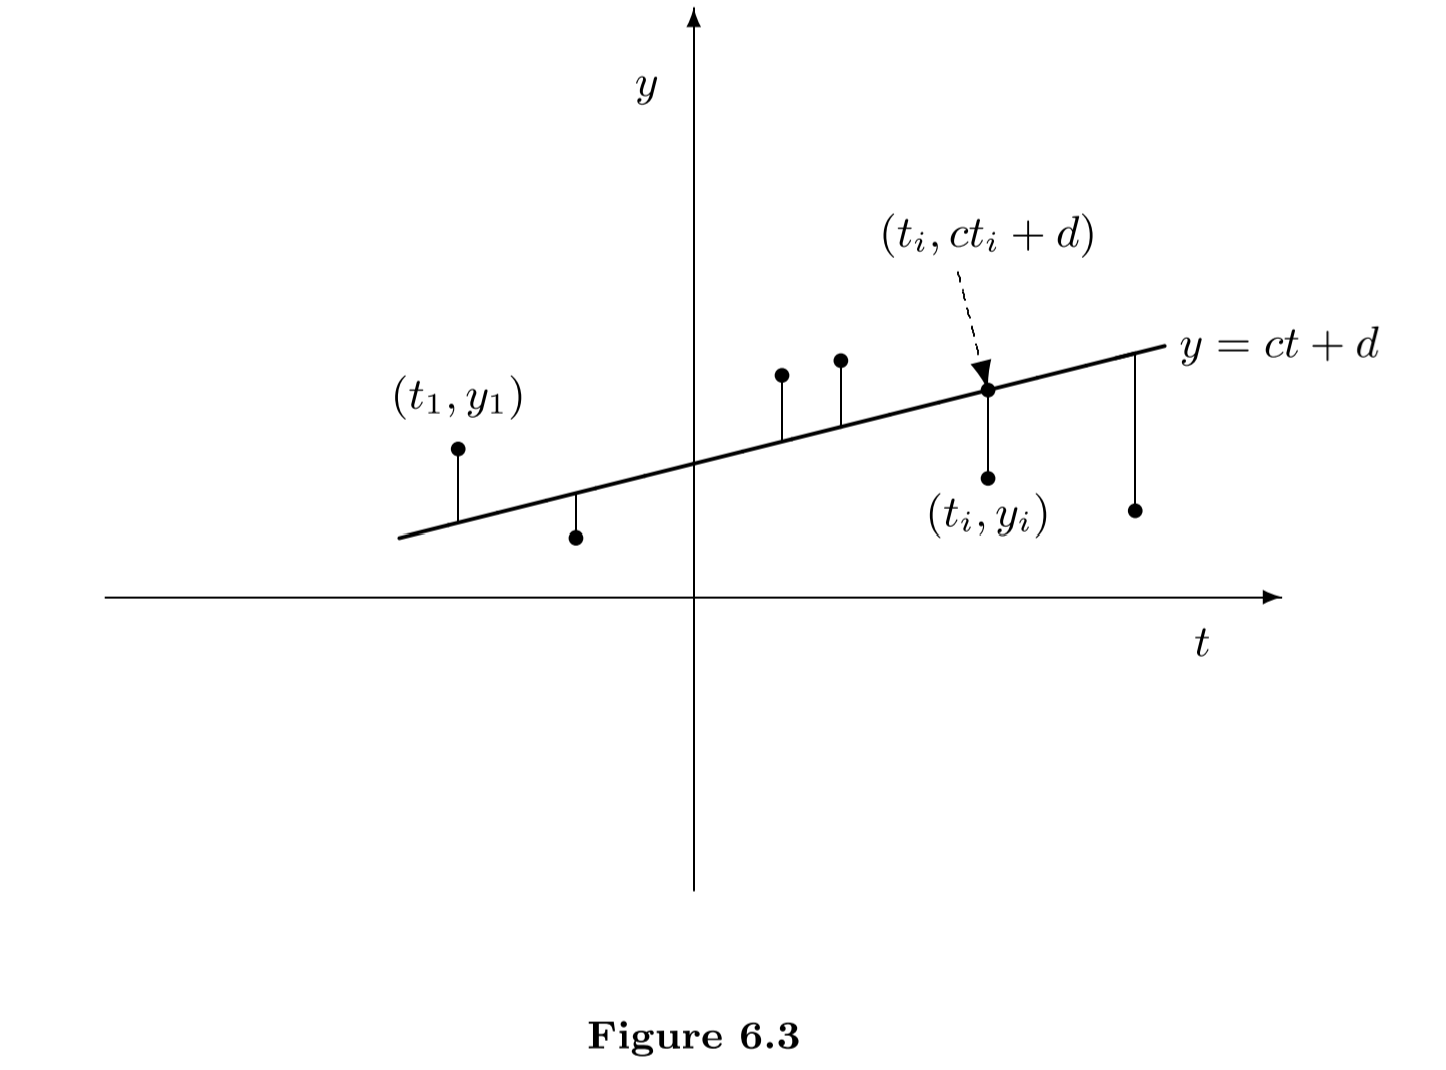
\includegraphics[width=12cm]{images/figure-6-3.png}
\end{center}

Thus the problem is reduced to finding the constants \(c\) and \(d\) that \emph{minimize} \(E\).
(For this reason the line \(y = ct + d\) is called the \textbf{least squares line}.)
If we let
\[
    A = \begin{pmatrix} t_1 & 1 \\ t_2 & 1 \\ \vdots & \vdots \\ t_m & 1 \end{pmatrix}, \quad x = \begin{pmatrix} c \\ d \end{pmatrix}, \quad \text{and} \quad y = \begin{pmatrix} y_1 \\ y_2 \\ \vdots \\ y_m \end{pmatrix},
\]
then it follows that \(E = \norm{y - Ax}^2\).

We develop a \emph{general} method for finding an explicit vector \(x_0 \in F^n\) that minimizes \(E\);
that is, given an \(m \X \RED{n}\) matrix \(A\), we find \(x \in F^{\RED{n}}\) such that \(\norm{y - Ax_0} \le \norm{y - Ax}\) for all vectors \(x \in F^{\RED{n}}\).
In this case \(A\) is \(m \X 2\) matrix and \(x_0 \in F^2\).
But this method not only allows us to find the linear function that best fits the data, but also, for any positive integer \(k\), the best fit using a polynomial of degree at most \(k\).
(And in that case, the matrix a will be \(m \X (k + 1)\) and \(x_0 \in F^{k + 1}\).)

First, we need some notation and two simple lemmas.
For \(x, y \in F^n\), let \(\LG x, y \RG_{\RED{n}}\) denote the \emph{standard} inner product of \(x\) and \(y\) in \(F^{\RED{n}}\).

\begin{remark} \label{remark 6.3.6}
Recall that if \(x\) and \(y\) are regarded as \emph{column vectors}, then \(\LG x, y \RG_n = y^*x\).
\end{remark}

\begin{lemma} \label{lem 6.1}
Let \(A \in M_{m \X n}(F)\), \(x \in F^{\MAROON{n}}\) and \(y \in F^{\RED{m}}\).
Then
\[
    \LG Ax, y \RG_{\RED{m}} = \LG x, A^*y \RG_{\MAROON{n}}.
\]
\end{lemma}

\begin{note}
這個\ lemma 跟\ \THM{6.9} 很像,就是把\ \(A\) 從左搬到右時需要加\ star。但跟\ \THM{6.9} 差別就在於內積空間的維度要跟著變。
\end{note}

\begin{proof}
Proof. By a generalization of the \CORO{6.11.1}(see \EXEC{6.3.5}(b)), we have
\begin{align*}
    \LG Ax, y \RG_{\RED{m}} & = y^* Ax & \text{by \RMK{6.3.6}} \\
        & = (y^* A) x & \text{by ``matrix'' associativity} \\
        & = (y^* A^{**}) x & \text{by generalization of \CORO{6.11.1}(d)} \\
        & = (A^* y)^* x & \text{by generalization of \CORO{6.11.1}(c)} \\
        & = \LG x, A^* y \RG_{\MAROON{n}} & \text{by \RMK{6.3.6} again}
\end{align*}
\end{proof}

\begin{lemma} \label{lem 6.2}
Let \(A \in M_{m \X n}(F)\).
Then \(\rank(A^* A) = \rank(A)\).
\end{lemma}

\begin{proof}
By the dimension theorem, it suffices to show that \(\NULL(A) = \NULL(A^* A)\), and to show that we can show, for \(x \in F^n\), we have \(A^* Ax = 0_{_{F^n}}\) if and only if \(Ax = 0_{_{F^m}}\).

Clearly, the \(\Longleftarrow\) direction is true, that is, \(Ax = 0_{_{F^m}}\) implies that \(A^* Ax = A^* 0_{_{F^m}} = 0_{_{F^n}}\).
So we show the \(\Longrightarrow\), that is, assume that \(A^* A x = 0_{_{F^n}}\).
Then
\begin{align*}
    0 & = \LG 0_{_{F^n}}, x \RG_n & \text{by \THM{6.1}(c)} \\
      & = \LG A^* A x, x \RG_n & \text{by supposition} \\
      & = \LG A x, A^{**} x \RG_m & \text{by \LEM{6.1}} \\
      & = \LG A x, A x \RG_m & \text{by generalization of \CORO{6.11.1}(d)}
\end{align*}
Then by \THM{6.1}(d), \(Ax = 0_{_{F^m}}\), as desired.
\end{proof}

\begin{lemma} \label{lem 6.3}
(This is in fact the corollary behind the lemma 2, but I cannot give index for such kind of corollary, so I rename it as lemma 3.)
If \(A\) is an \(m \X n\) matrix such that \(\rank(A) = n\), then \(A^* A\), by \LEM{6.2}, also has rank \(n\), and is an \(n \X n\) matrix, hence is invertible.
\end{lemma}

Now let \(A\) be an \(m \X n\) matrix and \(y \in F^{\RED{m}}\).
Define \(\W = \{ Ax : x \in F^n \}\); that is, \(\W = \RANGE(\LMTRAN_A) \subseteq F^{\RED{m}}\).
By the \CORO{6.6.1}, there \emph{exists} a \textbf{unique} vector in \(\W\) that is ``closest'' to \(y\).
Call this vector \(Ax_0\), where \(x_0 \in F^n\).
Then \(\norm{Ax_0 - y} \le \norm{Ax - y}\) for all \(x \in F^n\); so \(x_0\) has the property that \(E = \norm{Ax_0 - y}\) is minimal, as desired.

\begin{remark} \label{remark 6.3.7}
Well, this argument is just a lifehack: we can of course use \CORO{6.6.1} to find that unique vector \(w \in \W\), but we need to do additional computation to decompose \(w\) as \(A x_0\), as described below.
\end{remark}

To develop a \emph{practical} method for finding such an \(x_0\), we note from \THM{6.6} and \CORO{6.6.1} that \textbf{\(A x_0 - y \in \W^{\perp}\)};
so since for all \(x \in F^n\), \(Ax \in \W\), and \(A x_0 - y \in \W^{\perp}\), we have \(\LG Ax, A x_0 - y \RG_m = 0\).
Thus, by \LEM{6.1}, we have that \(\LG Ax, A x_0 - y \RG_m = \LG x, A^*(Ax_0 - y) \RG_n = 0\) for all \(x \in F^n\);
that is, by \THM{6.1}(e), \(A^*(Ax_0 - y) = 0_{_{F^n}}\).
So we need only find \emph{a} solution \(x_0\) to \(A^* Ax = A^*y\), and \emph{despite of its terrible looking, it's just system of linear equations}, where \(A\) (hence \(A^*\)) and \(y\) are given.

If, in addition, we assume that \(rank(A) = n\), then by \LEM{6.3} \(A^* A\) is invertible, so multiplying the equation by \((A^* A)^{-1}\) we have \(x_0 = (A^* A)^{-1} A^*y\).
We summarize this discussion in the following theorem.

\begin{theorem} \label{thm 6.12}
Let \(A \in M_{m \X n}(F)\) and \(y \in F^m\).
Then there exists \(x_0 \in F^n\) such that \((A^* A)x_0 = A^*y\) and \(\norm{A x_0 - y} \le \norm{Ax - y}\) for all \(x \in F^n\).
Furthermore, if \(\rank(A) = n\), then \(x_0 = (A^* A)^{-1} A^* y\).

The proof is the long discussion above.
\end{theorem}

To return to our experimenter, let us suppose that the data collected are \((1, 2), (2, 3), (3, 5)\), and \((4, 7)\).
Then
\[
    A = \begin{pmatrix} 1 & 1 \\ 2 & 1 \\ 3 & 1 \\ 4 & 1 \end{pmatrix}
    \quad \text{ and } \quad y = \begin{pmatrix} 2 \\ 3 \\ 5 \\ 7 \end{pmatrix};
\]
In particular, \(A\) has rank \(2\), which is equal to its column size, hence \(A^* A\) is invertible.

And
\[
    A^* A =
    \begin{pmatrix} 1 & 2 & 3 & 4 \\ 1 & 1 & 1 & 1 \end{pmatrix}
    \begin{pmatrix} 1 & 1 \\ 2 & 1 \\ 3 & 1 \\ 4 & 1 \end{pmatrix}
    = \begin{pmatrix} 30 & 10 \\ 10 & 4 \end{pmatrix}
\]
Thus
\[
    (A^* A)^{-1} = \frac{1}{20} \begin{pmatrix}
        4 & -10 \\ -10 & 30
    \end{pmatrix}.
\]
Therefore by \THM{6.12},
\[
    \begin{pmatrix} c \\ d \end{pmatrix} = x_0
    = (A^* A)^{-1} A^* y
    = \frac{1}{20} \begin{pmatrix}
        4 & -10 \\ -10 & 30
    \end{pmatrix}
    \begin{pmatrix} 1 & 2 & 3 & 4 \\ 1 & 1 & 1 & 1 \end{pmatrix}
    \begin{pmatrix} 2 \\ 3 \\ 5 \\ 7 \end{pmatrix}
    = \begin{pmatrix} 1.7 \\ 0 \end{pmatrix}.
\]
It follows that the line \(y = 1.7t\) is the least squares line.
The error \(E\) may be computed directly as \(\norm{Ax_0 - u}^2 = 0.3\).

Suppose that the experimenter chose the times \(t_i (1 \le i \le m\)) to satisfy
\[
    \sum_{i = 1}^m t_i = 0.
\]
(But what context makes this case reasonable?)
Then (from the structure of \(A\) that, since the last column has all \(1\)'s,) the two columns of \(A\) would be not only \LID{} but also \emph{orthogonal}, hence by \EXEC{6.3.19}, so \(A^*A\) would be a \emph{diagonal} matrix.

In practice, the \(m \X 2\) matrix \(A\) in our least squares application has rank equal to two (since usually we will have \(t_i \ne t_j\) for some \(1 \le i, j \le m\)), and hence \(A^* A\) is invertible by \LEM{6.3}.
For, otherwise, the first column of \(A\) is a multiple of the second column, which consists only of ones.
But this would occur only if the experimenter collects all the data \emph{at exactly one time}, which makes little sense.

Finally, the method above may also be applied if, for some \(k\), the experimenter wants to fit a \emph{polynomial of degree at most \(k\)} to the data.
For instance, if a polynomial \(y = ct^2 + dt + e\) of degree at most \(2\) is desired, the appropriate model is
\[
    x = \begin{pmatrix} c \\ d \\ e \end{pmatrix}, \quad 
    y = \begin{pmatrix} y_1 \\ y_2 \\ \vdots \\ y_m \end{pmatrix}, \quad \text{ and } \quad
    A = \begin{pmatrix}
        t_1^2 & t_1 & 1 \\
        \vdots & \vdots & \vdots \\ 
        t_1^2 & t_1 & 1 \\
    \end{pmatrix}
\]
(BTW, If we just let the polynomial to be degree \(m\), then this problem reduced to finding Lagrange polynomial!)

\begin{note}
實際上只要\ \(t_1, ..., t_m\) 全部都不一樣,而且\ \(n \le m\),則\ \(A\) 一定\ rank \(n\),因為\ \(A\) 的 columns 都線性獨立。
證明很單純:當\ \(t_1, ..., t_m\) 都不一樣時范德蒙矩陣的\ columns 都線性獨立;
in particular,\(A\) 的\ columns 是一個范德蒙矩陣的子集合,所以線性獨立。
\end{note}

\subsection{Minimal Solutions to Systems of linear Equations} \label{sec 6.3.2}

Even when a system of linear equations \(Ax = b\) is consistent, there may be no \emph{unique} solution.
In such cases, it may be desirable to find a solution of \textbf{minimal norm}.
A solution \(s\) to \(Ax = b\) is called a find a solution of \textbf{minimal norm} if \(\norm{s} \le \norm{u}\) for all other solutions \(u\).
The next theorem assures that every consistent system of linear equations has a \textbf{unique} minimal solution and provides a method for computing it.

\begin{theorem} \label{thm 6.13}
Let \(A \in M_{m \X n}(F)\) and \(b \in F^m\).
Suppose that \(Ax = b\) is consistent.
Then the following statements are true.
\begin{enumerate}
\item There exists \textbf{exactly one} minimal solution \(s\) of \(Ax = b\), and \(s \in \RANGE(\LMTRAN_{A^*})\).
\item The vector \(s\) is \textbf{the only solution} to \(Ax = b\) that \textbf{lies in} \(\RANGE(\LMTRAN_{A^*})\);
in fact, \(s = A^*u\) where \(u\) is any vector that satisfies \((AA^*)u = b\).
\end{enumerate}
\end{theorem}

\begin{proof} \ 

\begin{enumerate}
\item For simplicity of notation, we let \(\W = \RANGE(\LMTRAN_{A^*}) \subseteq F^n\) and \(\W' = \NULL(\LMTRAN_A) \subseteq F^n\).
Let \(x \in F^n\) be any solution to \(Ax = b\).
By \THM{6.6}, \(x = s + y\) for some \(s \in \W\) and \(y \in \W^{\perp}\).
\textbf{But} \(\W^{\perp} = \W'\) by \EXEC{6.2.12}, and therefore \(y \in \W' = \NULL(\LMTRAN_A)\), hence \(Ay = 0_{_{F^m}}\), hence \(b = Ax = A(s + y) = As + Ay = As + 0_{_{F^m}} = As\).
So \(s\) is also a solution to \(Ax = b\) and \(s\) lies in \(\W = \RANGE(\LMTRAN_{A^*})\).

To prove (a), we need only show that \(\RED{s}\) is the \emph{unique} and \emph{minimal} solution.
Let \(v\) be any solution to \(Ax = b\).
By \THM{3.9}, we have that \(v = \RED{s} + u\) \MAROON{(1)}, where \(u \in \NULL(\LMTRAN_A)\), that is \(u \in \W'\).
Since \(s \in \W\), which equals \(\W'^{\perp}\) by \EXEC{6.2.12} again (precisely, with \EXEC{6.2.13}(c)), we have
\begin{align*}
    \norm{v}^2 & = \norm{s + u}^2 & \text{by \MAROON{(1)}} \\
    & = \norm{s}^2 + \norm{u}^2 & \text{since \(s \in \W'^{\perp}\) and \(u \in \W'\),} \\
    & & \text{with \EXEC{6.1.10}} \\
    & \ge \norm{s}^2 & \text{of course}
\end{align*}
Thus \(s\) is a minimal solution.
We can also see from the preceding calculation that if \(\norm{v} = \norm{s}\), then \(\norm{u}^2 = 0\) hence \(u = 0_{_{F^n}}\); hence \(v = s + u = s + 0_{_{F^n}} = s\).
Therefore \(s\) is the \emph{unique minimal} solution to \(Ax = b\), proving (a).

\item
Assume that \(v\) is also a solution to \(Ax = b\) that \emph{lies in} \(\W\).
Then in particular, \(A(v - s) = Av - As = b - b = 0_{_{F^n}}\), so \(v - s\) is in \(\NULL(\LMTRAN_A)\);
that is, \(v - s \in \W'\).
So \(v, s \in \W\), \(v - s \in \W'\), we have \(v - s \in \W \cap \W'\).
But we have said (by \EXEC{6.2.12}) that \(\W' = \W^{\perp}\), hence \(v - s \in \W \cap \W^{\perp}\), which (by \EXEC{6.2.10}) is equal to \(\{ 0_{_{F^n}} \}\).
Hence \(v - s = 0_{_{F^n}}\) hence \(v = s\),
So \(s\) is the only solution that lies in \(\W\), that is, \(\RANGE(\LMTRAN_{A^*})\).

Finally, suppose that \((AA^*)u = b\) \MAROON{(2)}, and let \(v = A^*u.\).
Then in particular \(v \in \RANGE(\LMTRAN_{A^*})\), that is, \(v \in \W\), and by \MAROON{(2)} \(b = (A A^*)u = A (A^* u) = A v\).
Then by the discussion above, \(v\) is the only solution \(Ax = b\) and lies in \(\W = \RANGE(\LMTRAN_{A^*})\), hence we conclude that the unique minimum solution has the form \(s = v = A^*u\).
\end{enumerate}
\end{proof}

\begin{example} \label{example 6.3.3}
Consider the system
\[
    \sysdelim..\systeme{
        x + 2y + z = 4,
        x - y + 2z = -11,
        x + 5y = 19.
    }
\]
Let
\[
    A = \begin{pmatrix} 1 & 2 & 1 \\ 1 & -1 & 2 \\ 1 & 5 & 0 \end{pmatrix} \quad \text{ and } \quad
    b = \begin{pmatrix} 4 \\ -11 \\ 19 \end{pmatrix}.
\]
To find the minimal solution to this system, by \THM{6.13}(b), we must first find some solution \(u\) to the equation \(AA^*x = b\).
Now
\[
    AA^* = \begin{pmatrix}
        6 & 1 & 11 \\
        1 & 6 & -4 \\
        11 & -4 & 26
    \end{pmatrix};
\]
so we consider the system
\[
    \sysdelim..\systeme{
        6x + y + 11z = 4,
        x + 6y - 4z = -11,
        11x - 4y + 26z = 19\,
    }
\]
for which one solution is
\[
    u = \begin{pmatrix} 1 \\ -2 \\ 0 \end{pmatrix}.
\]
(Any solution will suffice.) Hence by \THM{6.13}(b),
\[
    s = A^* u = \begin{pmatrix} -1 \\ 4 \\ 3 \end{pmatrix}
\]
is the minimal solution to the given system.
\end{example}
